% 半角 例2：等腰直角△ABC，∠BAC=90°，AB=AC，D,E∈BC，∠DAE=45°，证 DE²=BD²+EC²
\documentclass[tikz,border=4pt]{standalone}
\usepackage{ctex}
\usepackage{amsmath}
\usetikzlibrary{calc, decorations.markings}
\begin{document}
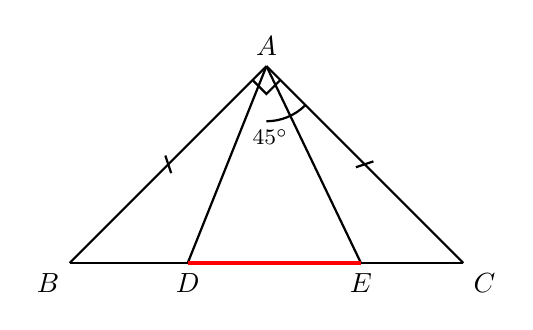
\begin{tikzpicture}[scale=1.0, thick,
  tick/.style={postaction={decorate, decoration={markings,
    mark=at position 0.5 with {\draw (-1.5pt,-3pt) -- (1.5pt,3pt);}}}}]
  % A 顶点直角，B 左 C 右
  \coordinate (A) at (0, 2.5);
  \coordinate (B) at (-2.5, 0);
  \coordinate (C) at (2.5, 0);
  \coordinate (D) at (-1, 0); % B 到 D
  \coordinate (E) at (1.2, 0);
  \draw[tick] (A)--(B);
  \draw[tick] (A)--(C);
  \draw (B)--(C);
  \draw (A)--(D);
  \draw (A)--(E);
  \draw[red, very thick] (D)--(E);
  % 直角符号 A
  \draw ($(A)+(-135:0.25)$) -- ($(A)+(-135:0.25)+(-45:0.25)$) -- ($(A)+(-45:0.25)$);
  % ∠DAE
  \draw ($(A)+(-90:0.7)$) arc[start angle=-90, end angle=-90+45, radius=0.7];
  % approx: AD dir from A: angle to D=(−1−0,0−2.5)=(-1,-2.5), atan2 ≈ -111.8°
  % AE dir: (1.2,-2.5), atan2 ≈ -64.4°
  \node at (0.05,1.6) {\footnotesize $45^\circ$};
  \node[above] at (A) {$A$};
  \node[below left] at (B) {$B$};
  \node[below right] at (C) {$C$};
  \node[below] at (D) {$D$};
  \node[below] at (E) {$E$};
\end{tikzpicture}
\end{document}
